%- explicar como se pretende tratar a variável de interesse... .

% quais caminhos são apontados até agora ...


\section{Tratamento da variável de interesse}

Como visto anteriormente, um dos principais problemas ao lidar com dados para fecundidade masculina é a qualidade da informação. Particularmente, quando falamos de registros administrativos, muitos países apresentam proporções altas de informação faltante para idade do pai, o que dificulta ou, por vezes, impossibilita o cálculo de taxas de fecundidade para os homens.

Uma abordagem proposta por alguns autores para o tratamento de dados faltantes para a variável idade do pai (\ref{bases_e_metodos-ref}), considera que a probabilidade da informação para a idade do pai ser ausente depende da idade da mãe. Como veremos adiante, na seção de métodos, existem diferentes pressupostos para a imputação de dados, que alteram os tipos de tratamentos que podem ser realizados para cada caso.  

\citeonline{dudel2019estimating}, por exemplo (explorado preliminarmente na seção \ref{bases_e_metodos-ref}), afirmam que a imputação condicional das idades paternas faltantes pelas idades observadas das mães tem um desempenho melhor para a estimação das TEFMs e TFTM do que uma imputação incondicional. Segundo os autores, a idade materna ao nascer é correlacionada tanto com idade paterna ao nascer, como com a probabilidade da idade do pai ser não observada. Para comprovar sua hipótese, os autores realizam simulações. 



\textcolor{red}{[complementar]}










\begin{comment}
    

Há uma probabilidade maior da idade paterna ser ausente entre mães mais jovens. Isso porque mães mais jovens teriam, majoritariamente, maior chance de serem mães solteiras. E, as mães mais jovens normalmente têm parceiros mais jovens. Logo, a distribuição dos valores omitidos seriam de pais mais jovens do que os pais com idade observada \cite{dudel2019estimating}. 

Observando a proporção de mães em cada ano e faixa etária que possuem idade do pai faltante para o estado do Rio de Janeiro, é possível visualizar que as faixas mais jovens possuem uma maior proporção de dados faltantes. O padrão mostra que, quanto mais jovens, maior a proporção de dado faltante na faixa etária. O gráfico \ref{graf:rj-conjulgal-mae} mostra que, no estado do Rio de Janeiro, a proporção das mulheres que, em cada situação conjugal e ano, tinham idade do pai faltante era maior entre as solteiras e mais baixas entre mães casadas ou em união estável, apesar de ainda serem proporções acima de 20\% em todo o intervalo.

\begin{grafico}
    \centering  
    \caption{Proporção de idade do pai ignorada em cada faixa etária da mãe e ano no estado do Rio de janeiro}
        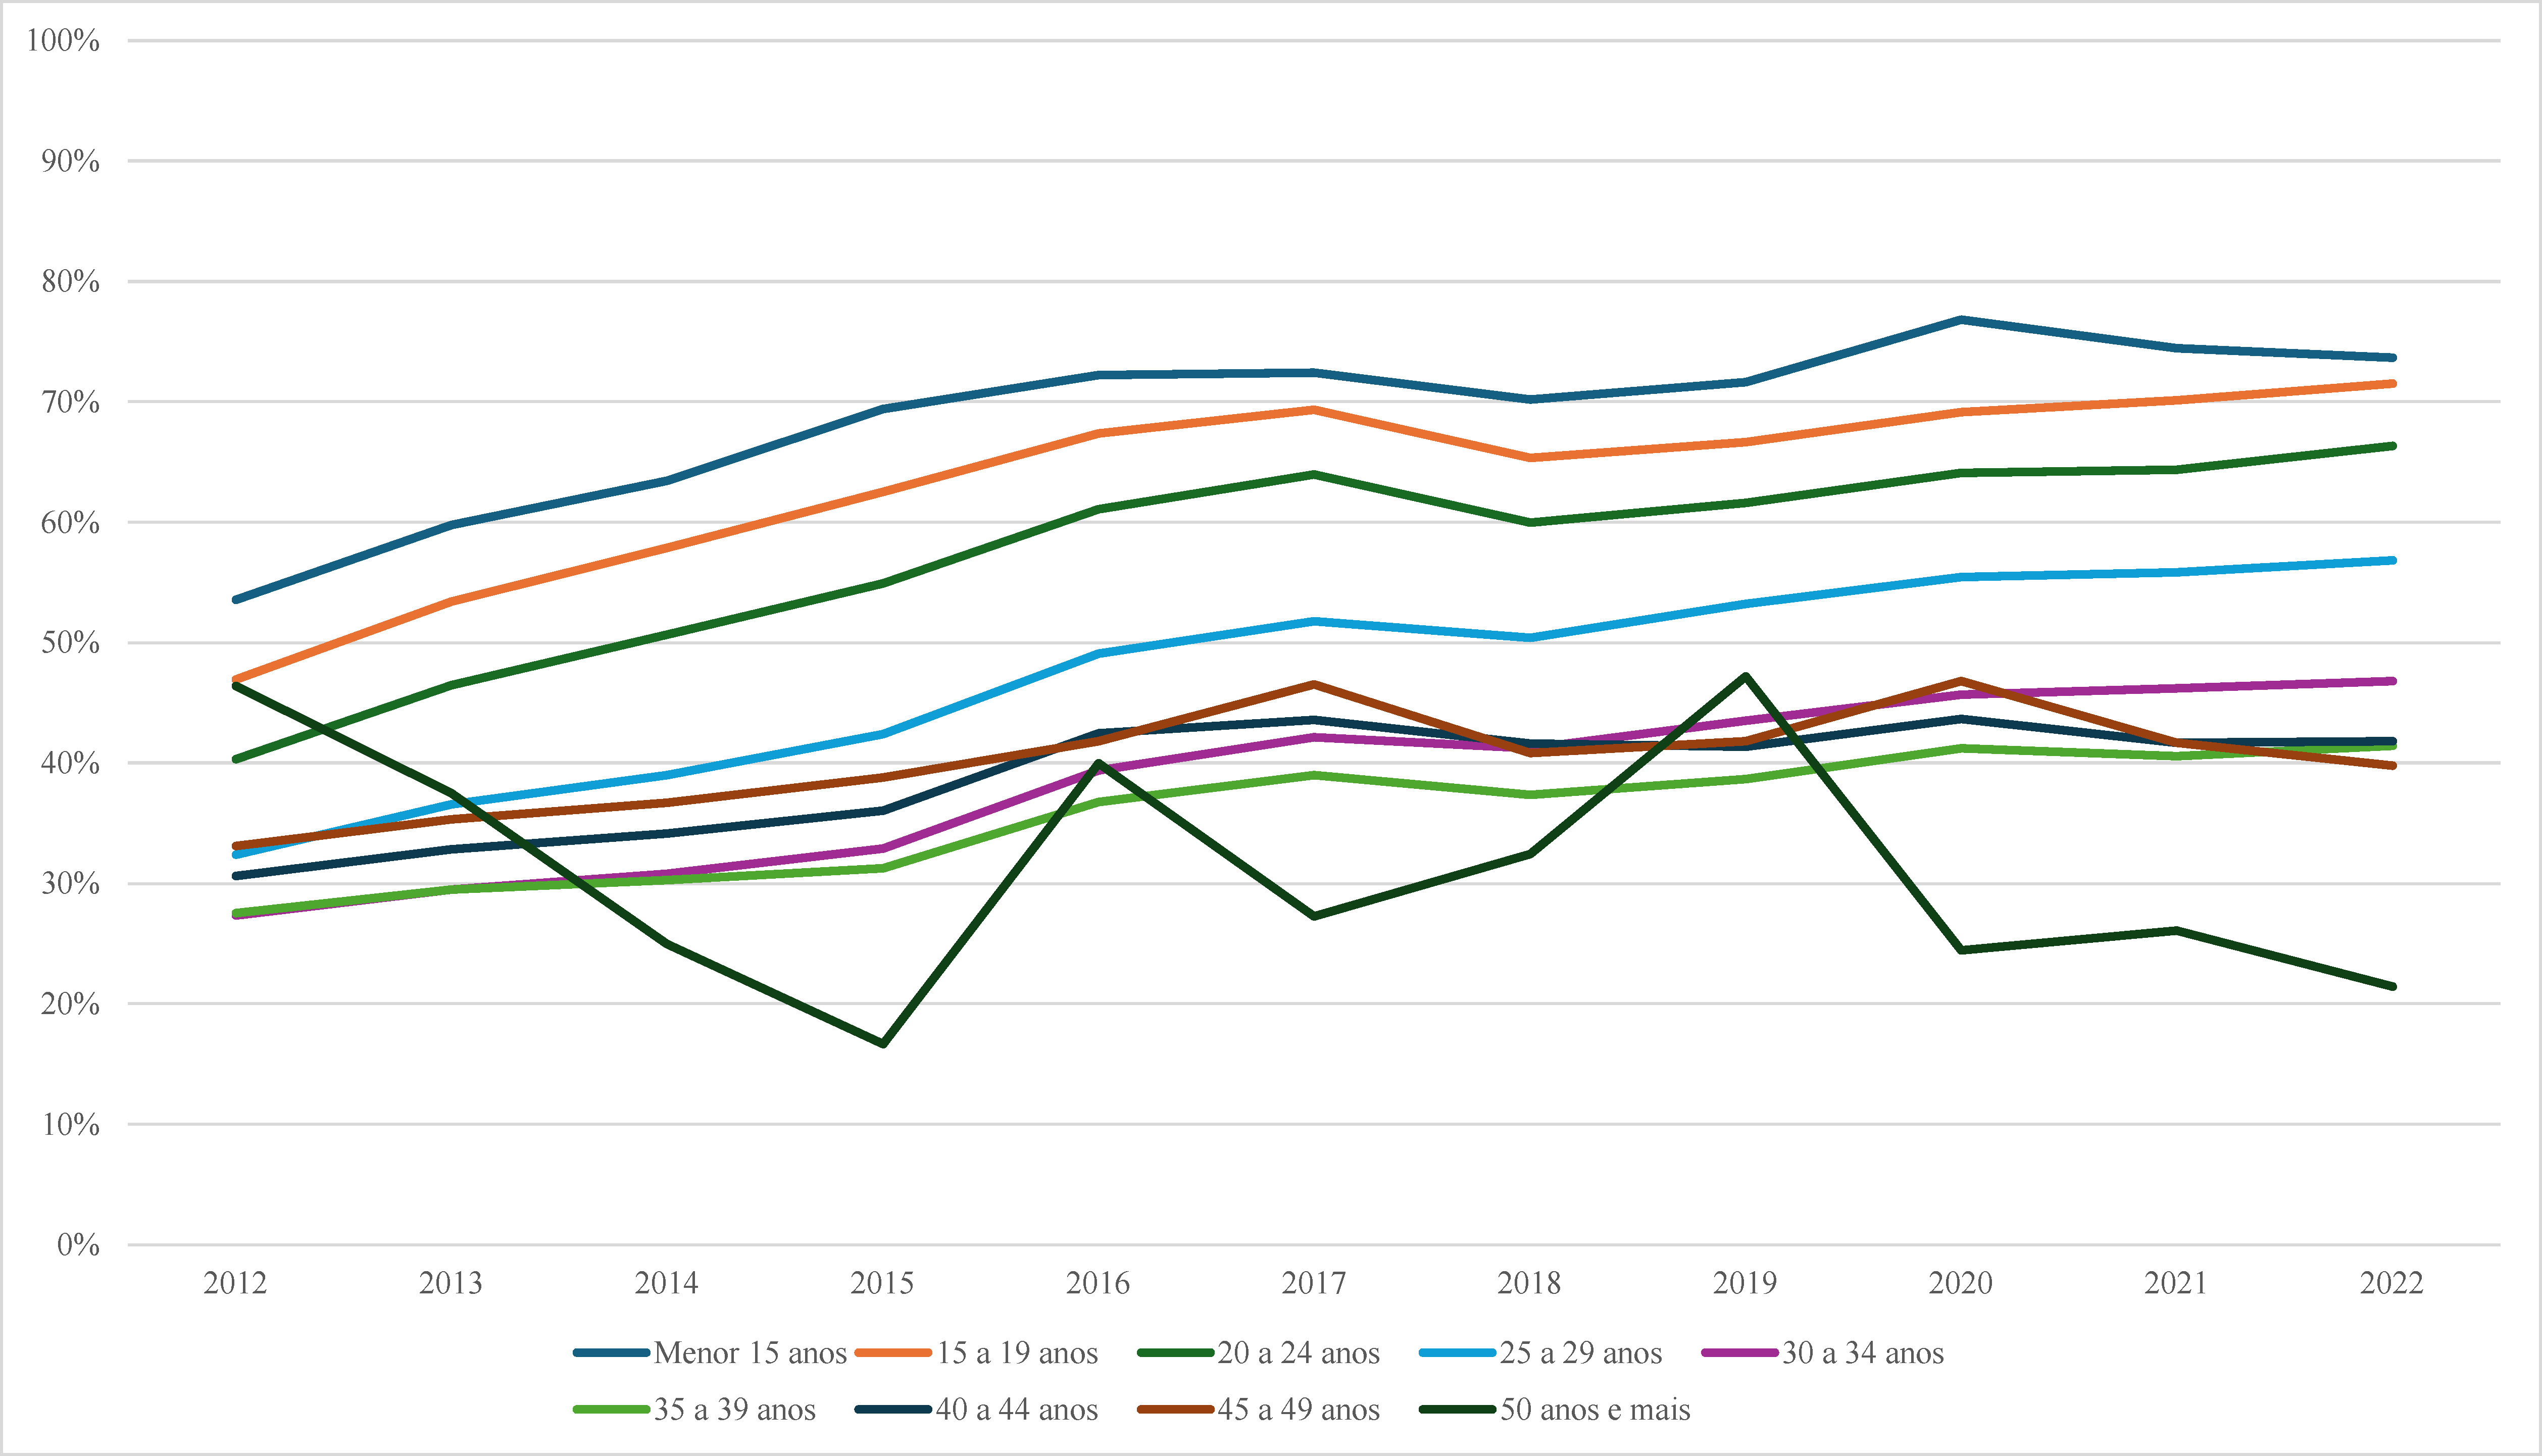
\includegraphics[width=5.0in]{imagens/Proporcao de idade do pai ignorada em cada faixa etaria da mae e ano.pdf}
    \fonte{Datasus - Sinasc - Informações de saúde RJ}
    \label{graf:ignorado-rj-faixa-etaria-mae}
\end{grafico}


\begin{grafico}
    \centering  
    \caption{Proporção das mães com idade do pai ignorada em cada ano e situação conjugal no estado do Rio de janeiro}
        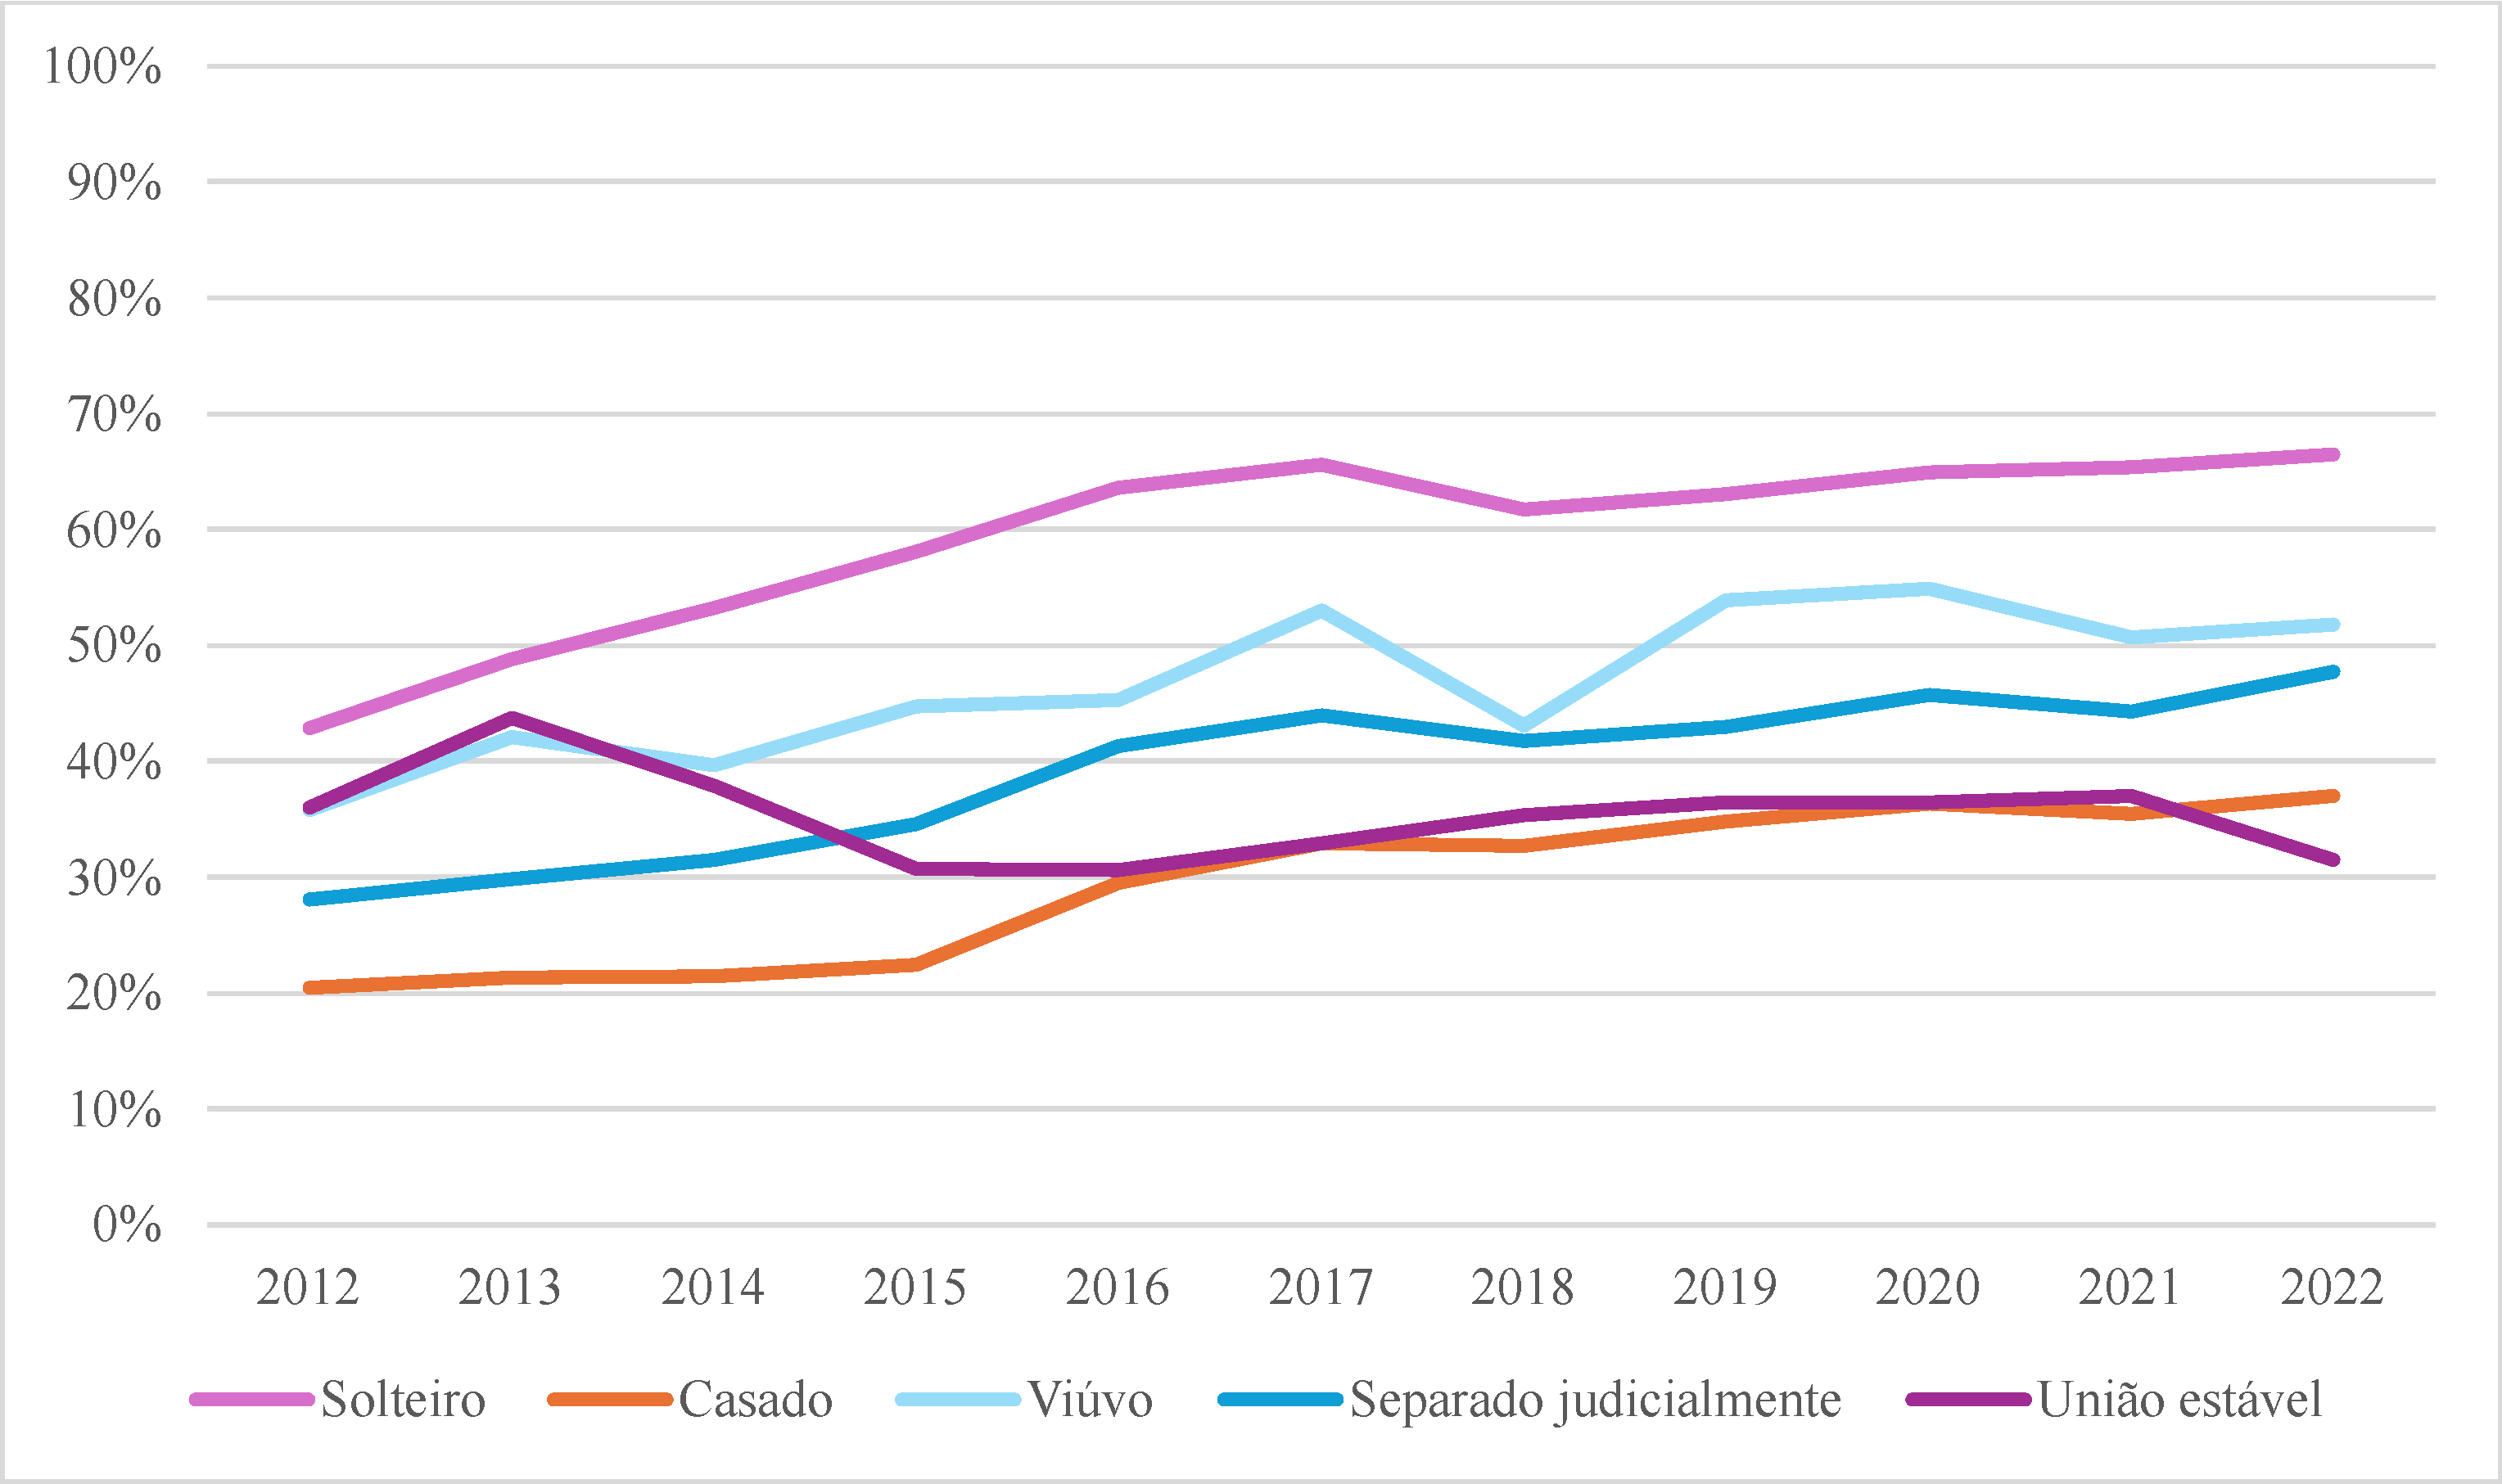
\includegraphics[width=5.0in]{imagens/Proporção das mães com idade do pai ignorada em cada ano e situação conjulgal.pdf}
    \fonte{Datasus - Sinasc - Informações de saúde RJ}
    \label{graf:rj-conjulgal-mae}
\end{grafico}


    \textbf{ratio of male to female TFRs (RTFRs)}
    
    \begin{equation}
        R_{TFT}= \frac{TFTM}{TFTF}
    \end{equation}
    

\end{comment}
